
\chapter{System analysis}

This chapter is about analysing the problem space more detailed, separating concerns\todo{cite?} and finding solutions in an architectural viewpoint.
It is important to find an architecture, that achieves all requirements and is able to evolve for upcoming changes.
In some areas where this is foreseeable, preparations to apply upcoming changes easier can be implemented, whereas in other regions this is not possible.
Generally, sticking to the SOLID\todo{.} and YAGNI\todo{.} principles, will help to achieve this goal.

\section{System Architecture}

The requirements listed in \autoref{requirements} will be used to draft an initial architecture.
By sorting these requirements, the following layers can be extracted: \todo{.}

\subsection{Layer 1: Orchestration Service}

This layer is all about the fundamental business logic: when to schedule, start and fail which stage of what project, while watching the hardware utilization.
This level is also responsible to coordinate these actions between all Winslow instances, so that there is no duplicate, missing or undetected node failure.

The following requirements are therefore implemented here: \todo{.?}

\subsection{Layer 2: Events and Resources}

For the first layer to communicate with the environment, such as reading configurations, project files or cooperation commands, this layer is essential.
It provides two important services: a synchronized event bus and a large file resource management.
The first is used to communicate with the other Winslow instances, while the latter is required for a stage execution.
Although list here as two separate services, they do not necessarily need to be backed up by two storages.
To provide a synchronized stream of events, it is required that the underlying storage provides some sort of synchronization primitives (see \todo{ref stream api / files?}).
The large file storage has no such requirement, as this is ensured by Winslow's stage synchronization and thus a eventual consistent\todo{cite} storage could be used here.

While knowing the different requirements, because of the time constraint of this thesis, a common NFS storage will be used\todo{autoref}.

\subsection{Layer 3: Backend Driver}

\subsection{Layer 4: REST API}

\subsection{Overview}

\begin{figure}[H]
	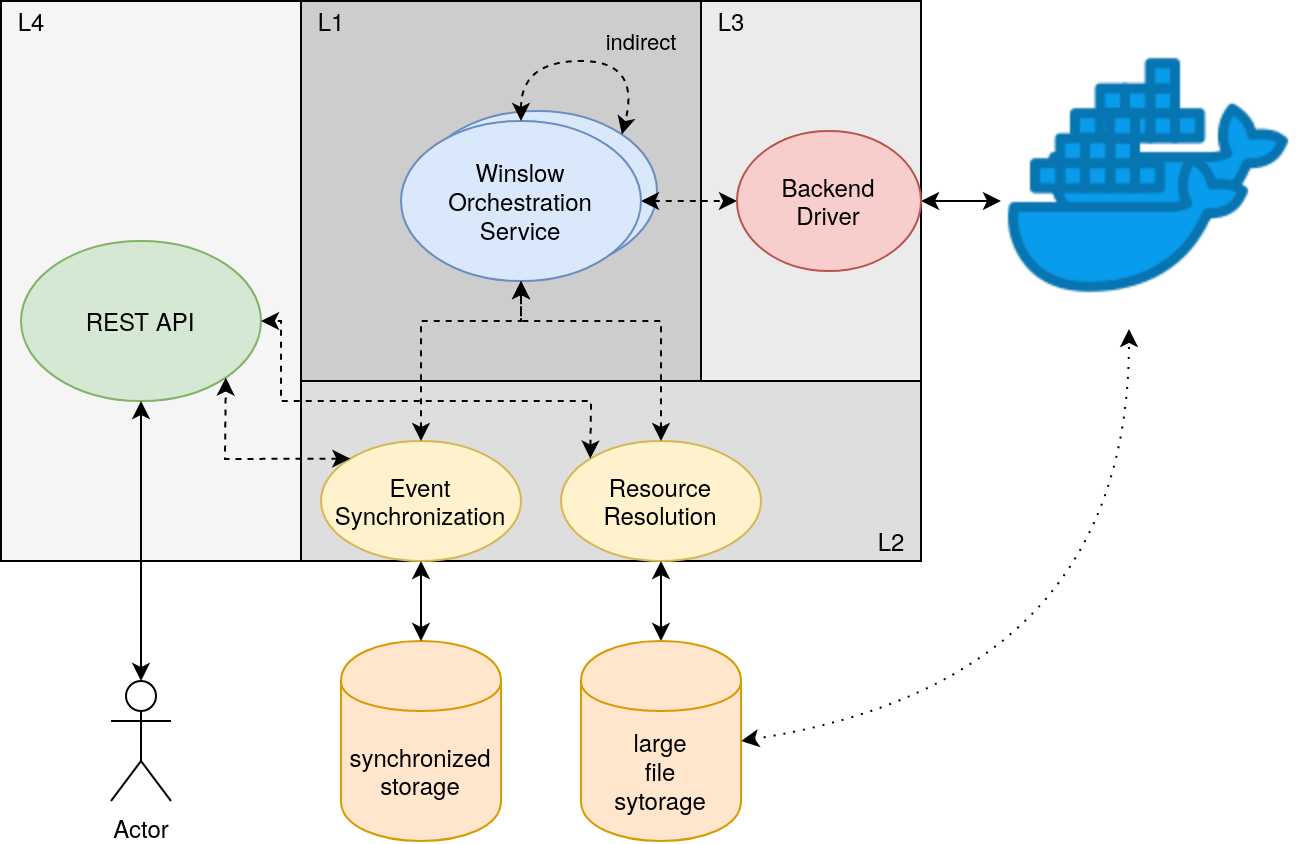
\includegraphics[width=0.99\textwidth]{architecture_detailed.png}
	\centering
	\caption{Architecture overview of a Winslow instance}
	\label{architecture:detailed}
\end{figure}

\todo{java interfaces for backend}

\todo{zwiebel layer model}

System Interacts with the User and other instances of itself

\begin{comment}
\section{Use Case Diagrams}
Finding all requirements can be challenging.
Drawing Use Case Diagrams can help to discover requirements while being very easy to understand.
This helps in understanding the customers needs \cite{Rosenberg2007} while the customer receives an impression on what will be reflected in the final product.

Listing all use cases in a single diagram negates the desired effect of it being easily understandable because of the number of interaction possibilities.
Instead, the interactions are grouped in categories and displayed in separate diagrams.
\autoref{use_case:overview} shows high-level use cases of all categories that are relevant to a user of the system.

\begin{figure}[H]
	\scalebox{.65}{
		\begin{tikzpicture}[node distance=5]
		\begin{umlsystem}{Winslow - Interaction Categories}
		\umlusecase[y=0,name=u1]{Manage Pipelines and Projects [\autoref{use_case:mgmt}]}
		\umlusecase[y=-1,name=u2]{Manage Resources and Workspaces [\autoref{use_case:files}]}
		\umlusecase[y=-2,name=u3]{Manage and Monitor Execution [\autoref{use_case:execution}]}
		\umlusecase[y=-3,name=u4]{Monitor Nodes [\autoref{use_case:monitor}]}
		\end{umlsystem}
		\umlactor[x=-9.5,y=-1.5]{User}
		\umlassoc{User}{u1}
		\umlassoc{User}{u2}
		\umlassoc{User}{u3}
		\umlassoc{User}{u4}
		\end{tikzpicture}
	}
	\centering
	\caption{Use Case Diagram showing the top level interaction categories}
	\label{use_case:overview}
\end{figure}

\subsection{Managing Pipelines and Projects}
\label{use_case:mgmt}

\todo{.}

\begin{figure}[H]
	\scalebox{.65}{
		\begin{tikzpicture}[node distance=5]
		\begin{umlsystem}{Winslow - Manage Pipelines and Projects}
		\umlusecase[y=0,name=u110]{\reqNameRef{mgmt:create:pipeline}}
		\umlusecase[y=-1,name=u120]{\reqNameRef{mgmt:update:pipeline}}
		\umlusecase[y=-2,name=u130]{\reqNameRef{mgmt:delete:pipeline}}
		\umlusecase[y=-3,name=u140]{\reqNameRef{mgmt:list:pipeline}}
		
		\umlusecase[y=-5,name=u210]{\reqNameRef{mgmt:create:project}}
		\umlusecase[y=-6,name=u220]{\reqNameRef{mgmt:update:project:pipeline}}
		\umlusecase[y=-7,name=u230]{\reqNameRef{mgmt:update:project:name}}
		\umlusecase[y=-8,name=u240]{\reqNameRef{mgmt:update:project:labels}}
		\umlusecase[y=-9,name=u250]{\reqNameRef{mgmt:delete:project}}
		\umlusecase[y=-10,name=u260]{\reqNameRef{mgmt:list:project}}
		\end{umlsystem}
		\umlactor[x=-9.5,y=-4]{User}
		\umlassoc{User}{u110}
		\umlassoc{User}{u120}
		\umlassoc{User}{u130}
		\umlassoc{User}{u140}
		\umlassoc{User}{u210}
		\umlassoc{User}{u220}
		\umlassoc{User}{u230}
		\umlassoc{User}{u240}
		\umlassoc{User}{u250}
		\umlassoc{User}{u260}
		\end{tikzpicture}
	}
	\centering
	\caption{Use Case Diagram showing the general management interactions}
\end{figure}


\subsection{Managing Resources and Workspaces}
\label{use_case:files}

\todo{.}

\begin{figure}[H]
	\scalebox{.65}{
		\begin{tikzpicture}[node distance=5]
		\begin{umlsystem}{Winslow - Manage Resources and Workspaces}
		\umlusecase[y=0,name=u110]{\reqNameRef{files:upload}}
		\umlusecase[y=-1,name=u120]{\reqNameRef{files:download}}
		\umlusecase[y=-2,name=u130]{\reqNameRef{files:list}}
		\end{umlsystem}
		\umlactor[x=-9.5,y=-1]{User}
		\umlassoc{User}{u110}
		\umlassoc{User}{u120}
		\umlassoc{User}{u130}
		\end{tikzpicture}
	}
	\centering
	\caption{Use Case Diagram showing the general management interactions}
\end{figure}

\subsection{Managing and Monitoring Executions}
\label{use_case:execution}

\todo{.}

\begin{figure}[H]
	\scalebox{.65}{
		\begin{tikzpicture}[node distance=5]
		\begin{umlsystem}{Winslow - Manage and Monitor Executions}
		\umlusecase[y=0,name=u110]{\reqNameRef{exec:start:stage}}
		\umlusecase[y=-1,name=u120]{\reqNameRef{exec:pause:stage}}
		\umlusecase[y=-2,name=u130]{\reqNameRef{exec:resume:stage}}
		\umlusecase[y=-3,name=u140]{\reqNameRef{exec:abort:stage}}
		\umlusecase[y=-5,name=u150]{\reqNameRef{exec:inspect:logs}}
		\umlusecase[y=-6,name=u160]{\reqNameRef{exec:inspect:state}}
		\end{umlsystem}
		\umlactor[x=-9.5,y=-3]{User}
		\umlassoc{User}{u110}
		\umlassoc{User}{u120}
		\umlassoc{User}{u130}
		\umlassoc{User}{u140}
		\umlassoc{User}{u150}
		\umlassoc{User}{u160}
		\end{tikzpicture}
	}
	\centering
	\caption{Use Case Diagram showing the general management interactions}
\end{figure}

\subsection{Monitoring Nodes}
\label{use_case:monitor}
\todo{.}
\begin{figure}[H]
	\scalebox{.65}{
		\begin{tikzpicture}[node distance=5]
		\begin{umlsystem}{Winslow - Monitor Nodes}
		\umlusecase[y=0,name=u110]{\reqNameRef{node:monitor:cpu}}
		\umlusecase[y=-1,name=u120]{\reqNameRef{node:monitor:ram}}
		\umlusecase[y=-2,name=u130]{\reqNameRef{node:monitor:netio}}
		\end{umlsystem}
		\umlactor[x=-9.5,y=-1]{User}
		\umlassoc{User}{u110}
		\umlassoc{User}{u120}
		\umlassoc{User}{u130}
		\end{tikzpicture}
	}
	\centering
	\caption{Use Case Diagram showing the general management interactions}
\end{figure}


\subsection{System Administration}

Furthermore to the interactions with a user, the system must provide further capabilities that are \todo{of} concern to the administrator.


\begin{figure}[H]
	\scalebox{.65}{
		\begin{tikzpicture}[node distance=5]
		\begin{umlsystem}{Winslow - Administration}
		\umlusecase[y=0,name=u1]{Start and Add a new Node}
		\umlusecase[y=-2,name=u2]{Stop and Remove a Node}
		\umlusecase[y=-4,name=u3]{Debug behavior of a Node}
		\end{umlsystem}
		\umlactor[x=-9.5,y=-2]{Admin}
		\umlassoc{Admin}{u1}
		\umlassoc{Admin}{u2}
		\umlassoc{Admin}{u3}
		\end{tikzpicture}
	}
	\centering
	\caption{Use Case Diagram showing administrative interactions}
	\label{use_case:admin}
\end{figure}
\end{comment}

\section{Communication / message analysis ?}

\section{Interface analysis}